The MMB 3.0 can be downloaded from \url{macromodelbase.com/download}. The version for windows is \texttt{mmb-electron-win.exe}, for macOS it is \texttt{mmb-electron-mac.dmg}, and for Linux directly download the source code from the release on github at
\url{https://github.com/IMFS-MMB/mmb-gui-electron/tags}.\footnote{Linux users will have to build from source using \texttt{npm}. Find more info on our github page.}
The Windows version and the Mac version of the file autoinstall the MMB on your computer and opens the redesigned frontend of the MMB. 

The files for carrying out the simulations of the models are written in MATLAB, so either some version of MATLAB or a recent version of its freeware clone, OCTAVE, must be installed on your computer. In the case of Matlab, one needs as well the \textit{Optimization Toolbox} as well as the \textit{Statistics Toolbox} in order to be able to run all models in the Modelbase.\footnote{For the time being there are some models, which cannot be simulated with Octave. The list of models contains: NK\_ET14, NK\_FLMF18, NK\_GK11, US\_AJ16, US\_CMR14, US\_CMR14noFa, US\_FRB08, US\_FRB08mx, US\_IR15, EA\_Q14. The problems with the latter model exist only with Octave 4.4.0.}
For model solution the program utilizes DYNARE, which can be downloaded free of charge from the web.\footnote{\url{http://www.dynare.org}} Under Windows, double-clicking on the downloaded DYNARE exe-file opens a set of steps that guide you through the installation. Under macOS, locate the downloaded pkg-file in Finder, and Control-click the icon to select Open from the menu, thus creating an exception for the app to be installed. The installer will then guide you through the installation. To install Linux verison of Dynare please follow the instructions on the Dynare Wiki\footnote{The DYNARE Wiki install guide for Ubuntu and Debian can be found at \url{http://www.dynare.org/DynareWiki/InstallOnDebianOrUbuntu}}.

\subsection*{Compatibility}
We have tested the tested the MMB 3.0 with DYNARE 4.5.6 and 4.5.7. Earlier versions may work but have not been tested.\\
On Windows, DYNARE 4.5.6 is compatible with OCTAVE 4.4.0, whereas DYNARE 4.5.7 is compatible with OCTAVE 4.4.1. Both Dynare versions are compatible with  MATLAB R2007b and later. For macOS, the compatibility between DYNARE and MATLAB is the same. However, at the time of this release, the highest OCTAVE-supported version of DYNARE is 4.5.6 (compatible with OCTAVE 4.4.0 on macOS).\\


\subsection*{Further steps before running comparisons}
When using MATLAB, one has to add the DYNARE path to MATLAB. In order to do so, open MATLAB and choose \textit{Set path} from the \textit{File} menu. Use the option \textit{Add folder} and browse to the directory where you have installed DYNARE. The DYNARE subfolder that has to be added is called \textit{MATLAB}.

Before running simulations with the MMB, you need to specify whether you want to run the simulations in MATLAB or OCTAVE. In order to do so, click on settings on the upper-right corner of the MMB as shown in the Figure 'Settings'. It opens a window, in which you have the option either to let the program scan for versions of MATLAB and OCTAVE installed on your computer, or to search manually. If the scan finds more than one version of MATLAB or OCTAVE, you can choose from the list of programs in this subwindow.

\begin{figure}[H]%[htb]
\centering
\caption{\textsc{Settings}}
\vspace{0.2cm}
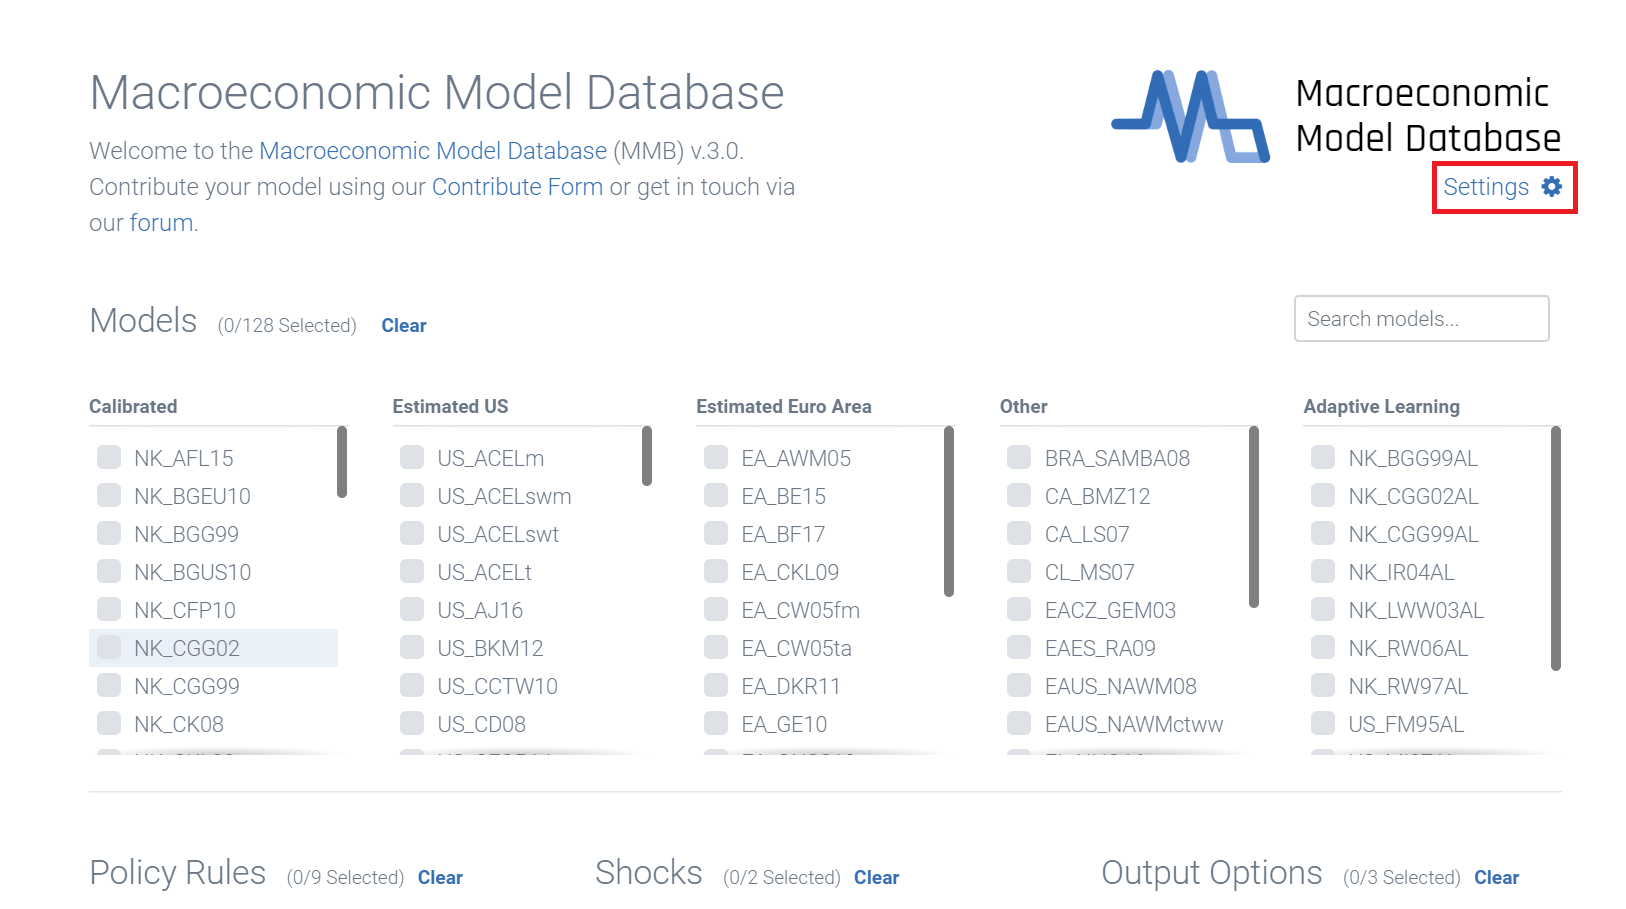
\includegraphics[width=12cm,keepaspectratio]{settings.png}\\[1cm]
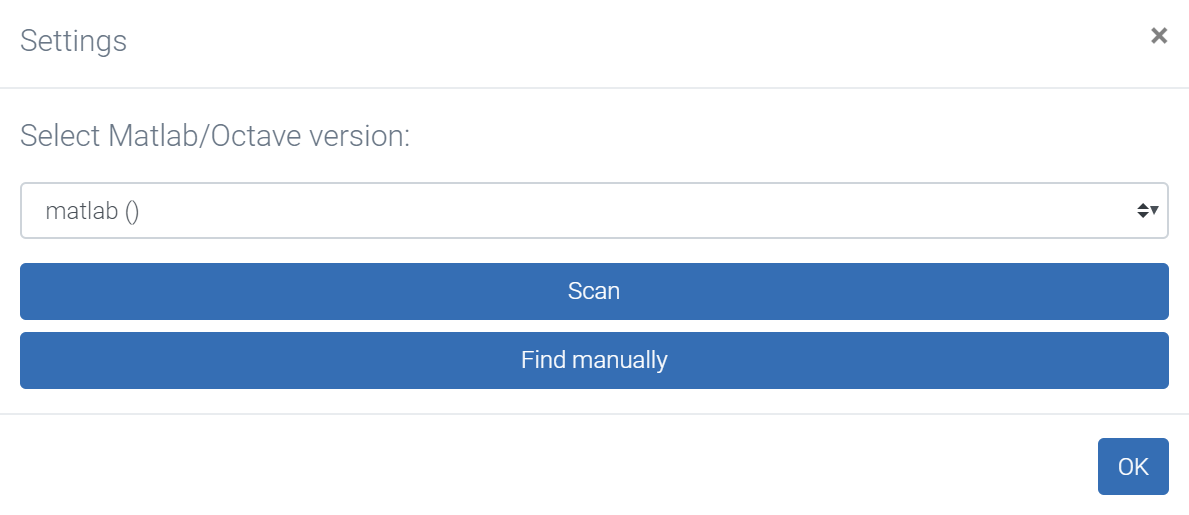
\includegraphics[width=9cm,keepaspectratio]{settings2.png}
\label{img:Settings}
\end{figure}






